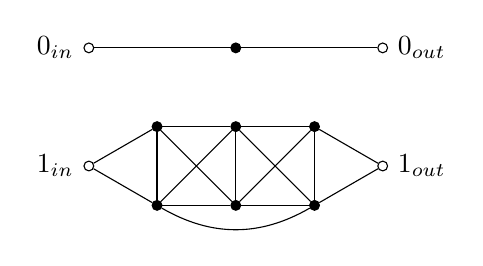
\begin{tikzpicture}
  [inner/.style={circle,draw=black!100,fill=black!100,inner sep = 1.25pt},
    attach/.style={circle,draw=black!100,fill=black!0,thin,inner sep = 1.25pt}]

  \node (0in) at (-1.866, 2) [attach, label=left:$0_{\text{in}}$] {};
  \node (0out) at (1.866, 2) [attach, label=right:$0_{\text{out}}$] {};
  \node at (0,2) [inner] {};

  \node (1) at (-1.866, .5) [attach, label=left:$1_{\text{in}}$] {};
  \node (2) at (1.866, .5) [attach, label=right:$1_{\text{out}}$] {};
  \node (3) at (-1      , 1) [inner] {};
  \node (4) at ( 0, 1) [inner] {};
  \node (5) at ( 1, 1) [inner] {};
  \node (6) at (-1, 0) [inner] {};
  \node (7) at (0 , 0) [inner] {};
  \node (8) at (1 , 0) [inner] {};

  \draw (0in) to (0out) [thin];

  \draw (1) to (3) [thin];
  \draw (1) to (6) [thin];
  \draw (2) to (5) [thin];
  \draw (2) to (8) [thin];
  \draw (3) to (4) [thin];
  \draw (3) to (6) [thin];
  \draw (3) to (7) [thin];
  \draw (4) to (5) [thin];
  \draw (4) to (6) [thin];
  \draw (4) to (7) [thin];
  \draw (4) to (8) [thin];
  \draw (5) to (7) [thin];
  \draw (5) to (8) [thin];
  \draw (6) to (7) [thin];
  \draw (7) to (8) [thin];
  \draw (6) to[out=330,in=210] (8) [thin];

\end{tikzpicture}